\documentclass{article}
\usepackage{tikz}
\usepackage[margin=.5in]{geometry}
\usetikzlibrary{shapes}
\begin{document}

\centerline{\sf Math/Econ 108: Epidemiology, Fall 2009}

\bigskip

\centerline{\bf An In-Class Simulation of the Spread of Disease}

\newcommand{\immuneCards}{
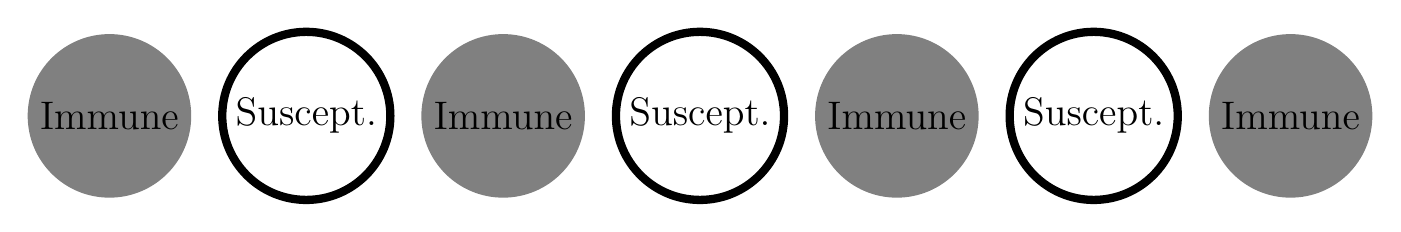
\begin{tikzpicture}
\node[minimum size=2cm,gray,fill,circle] at (-.8,0)  {\textcolor{black}{\Large Immune}};
\node[minimum size=2cm,circle,black,draw,line width=3pt] at (1.7,0)  {\textcolor{black}{\Large Suscept.}};
\node[minimum size=2cm,gray,fill,circle] at (4.2,0)  {\textcolor{black}{\Large Immune}};
\node[minimum size=2cm,circle,black,draw,line width=3pt] at (6.7,0)  {\textcolor{black}{\Large Suscept.}};\node[minimum size=2cm,gray,fill,circle] at (9.2,0)  {\textcolor{black}{\Large Immune}};
\node[minimum size=2cm,circle,black,draw,line width=3pt] at (11.7,0)  {\textcolor{black}{\Large Suscept.}};
\node[minimum size=2cm,gray,fill,circle] at (14.2,0)  {\textcolor{black}{\Large Immune}};
\end{tikzpicture}}

\newcommand{\infectCards}{

\begin{tikzpicture}[scale=1.2]
\node[minimum size=0cm,pink,fill,star] at (-3.5,0)  {\textcolor{black}{\parbox{.5in}{\centering Infect!\\North}}};
\node[minimum size=1.2cm,pink,fill,star] at (-0,0)  {\textcolor{black}{\parbox{.5in}{\centering Infect!\\South}}};
\node[minimum size=1.2cm,pink,fill,star] at (3.5,0)  {\textcolor{black}{\parbox{.5in}{\centering Infect!\\East}}};
\node[minimum size=1.2cm,pink,fill,star] at (7,0)  {\textcolor{black}{\parbox{.5in}{\centering Infect!\\West}}};
\end{tikzpicture}}

Each student gets one set of 4.   Cut them up and shuffle them.

\bigskip
\infectCards\\

\bigskip
\infectCards\\

\bigskip
\infectCards\\

\bigskip
\infectCards\\

\bigskip
\infectCards\\

\bigskip
\infectCards\\

\bigskip
\infectCards\\

\bigskip
\infectCards\\

\bigskip
\infectCards\\

\bigskip
\infectCards\\

\bigskip
\infectCards\\

\bigskip
\infectCards\\

\bigskip
\infectCards\\

\bigskip
\infectCards\\

\bigskip
\infectCards\\

\bigskip
\infectCards\\

\bigskip
\infectCards\\

\bigskip
\infectCards\\

\bigskip
\infectCards\\

\bigskip
\infectCards\\

\bigskip
\infectCards\\

\bigskip
\infectCards\\

\bigskip
\infectCards\\

\bigskip
\infectCards\\

\bigskip
\infectCards\\

\bigskip
\infectCards\\

\bigskip
\infectCards\\

\bigskip
\infectCards\\

\bigskip
\infectCards\\

\bigskip
\infectCards\\

\bigskip
\infectCards\\

\bigskip
\infectCards\\

\bigskip
\infectCards\\

\bigskip
\infectCards\\

\bigskip
\infectCards\\

\bigskip
\infectCards\\

\bigskip
\infectCards\\

\bigskip
\infectCards\\

\bigskip
\infectCards\\

\bigskip
\infectCards\\

\bigskip
\infectCards\\

\bigskip
\infectCards\\

\bigskip
\infectCards\\

\bigskip
\infectCards\\






\newpage

Whether you are immune.  Cut these up and put them in an envelope.  Each student takes one of the second simulation.

\bigskip

\noindent
\immuneCards\\
\bigskip
\immuneCards\\
\bigskip
\immuneCards\\
\bigskip
\immuneCards\\
\bigskip
\immuneCards\\
\bigskip
\immuneCards\\
\bigskip
\immuneCards\\
\bigskip

\newpage
State Cards.  Fold these so that you can keep track of your state:

\newcommand{\stateCard}{
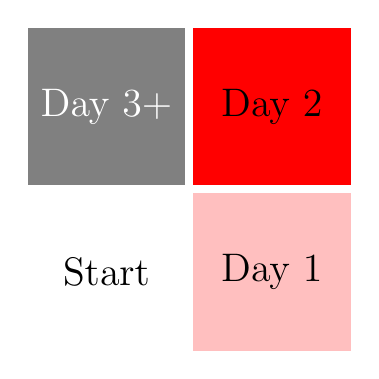
\begin{tikzpicture}
\node[minimum size=2cm] at (-2.1,0)  {\textcolor{black}{\Large Start}};
\node[minimum size=2cm,pink,fill] at (0,0)  {\textcolor{black}{\Large Day 1}};
\node[minimum size=2cm,red,fill] at (0,2.1)  {\textcolor{black}{\Large Day 2}};
\node[minimum size=2cm,gray,fill] at (-2.1,2.1)  {\textcolor{white}{\Large Day 3+}};
\end{tikzpicture}}

\bigskip
\noindent \stateCard \hspace*{.5in} \stateCard \hspace*{.5in} \stateCard\\

\bigskip
\noindent \stateCard \hspace*{.5in} \stateCard \hspace*{.5in} \stateCard\\

\bigskip
\noindent \stateCard \hspace*{.5in} \stateCard \hspace*{.5in} \stateCard\\

\bigskip
\noindent \stateCard \hspace*{.5in} \stateCard \hspace*{.5in} \stateCard\\

\bigskip
\noindent \stateCard \hspace*{.5in} \stateCard \hspace*{.5in} \stateCard\\

\bigskip
\noindent \stateCard \hspace*{.5in} \stateCard \hspace*{.5in} \stateCard\\

\bigskip
\noindent \stateCard \hspace*{.5in} \stateCard \hspace*{.5in} \stateCard\\

\bigskip
\noindent \stateCard \hspace*{.5in} \stateCard \hspace*{.5in} \stateCard\\

\bigskip
\noindent \stateCard \hspace*{.5in} \stateCard \hspace*{.5in} \stateCard\\

\bigskip
\noindent \stateCard \hspace*{.5in} \stateCard \hspace*{.5in} \stateCard\\

\bigskip
\noindent \stateCard \hspace*{.5in} \stateCard \hspace*{.5in} \stateCard\\

\bigskip
\noindent \stateCard \hspace*{.5in} \stateCard \hspace*{.5in} \stateCard\\

\bigskip
\noindent \stateCard \hspace*{.5in} \stateCard \hspace*{.5in} \stateCard\\

\bigskip
\noindent \stateCard \hspace*{.5in} \stateCard \hspace*{.5in} \stateCard\\

\bigskip
\noindent \stateCard \hspace*{.5in} \stateCard \hspace*{.5in} \stateCard\\


\end{document}